Taking the mask used in the previous section, we applied the “find edges” command of ImageJ. 
It uses a Sobel edge detector to highlight sharp changes in intensity in the active image or selection. 
Two $3 \times 3$ convolution kernels~\cite{edges} are used to generate vertical and horizontal derivatives.
The final image is produced by combining the two derivatives using the square root of the sum of the squares.

The main purpose of edge detection, in our case, is to improve the visualization of the lake's shrinking. 
Taking the edges of the lake in $1977$ and overlaying them to all the other images we were able to build a GIF that helps us to visualize in Fig. \ref{fig:edges} how much the lake retires with respect to its original size.
\begin{figure}[H]
    \centering
    \begin{subfigure}[b]{.45\textwidth}
        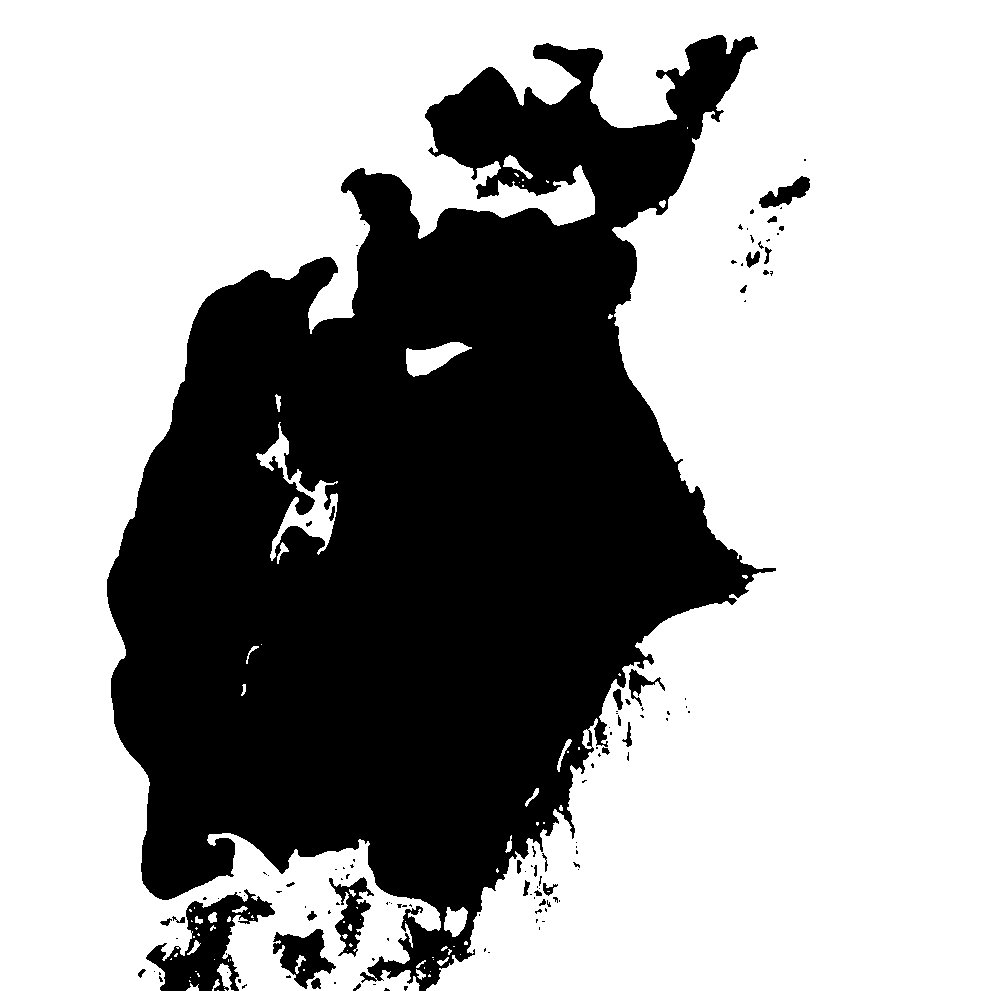
\includegraphics[width=\textwidth]{../img/mask.jpg}
        \caption{\emph{1977 mask.}}
    \end{subfigure}
    \begin{subfigure}[b]{.45\textwidth}
        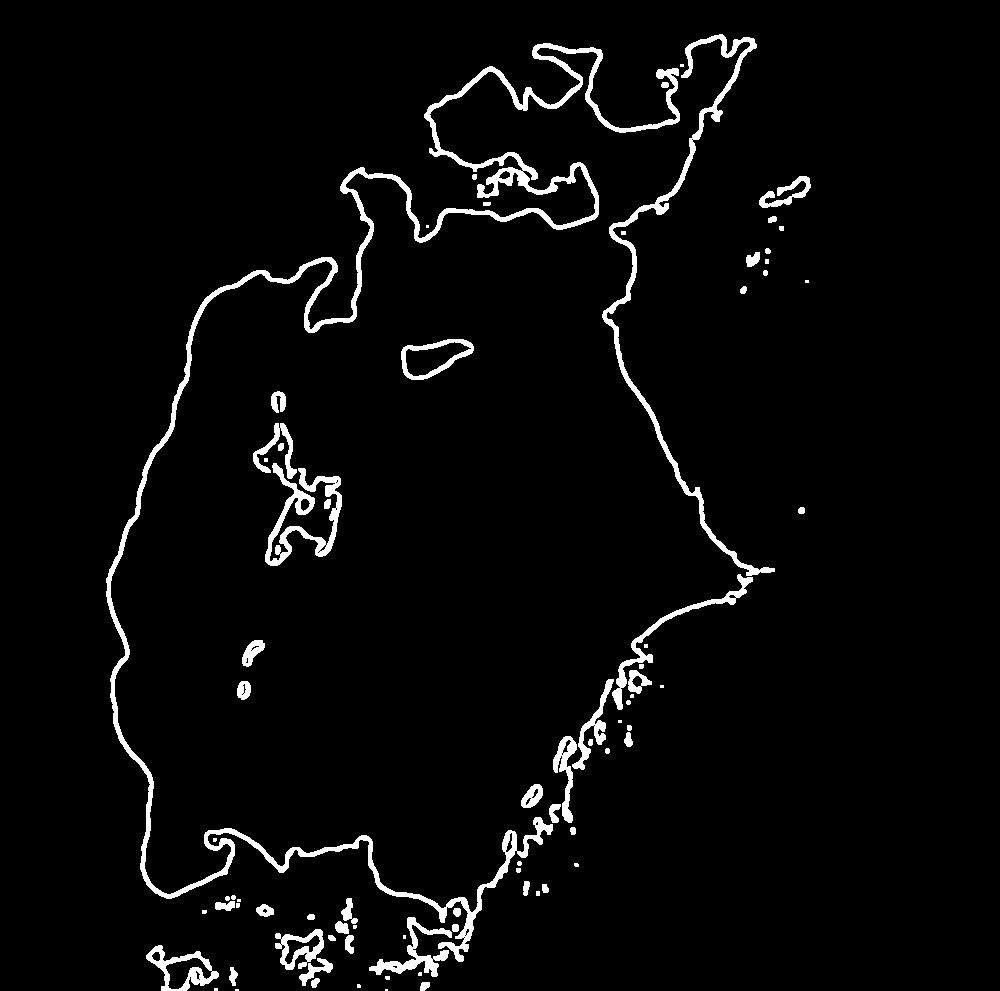
\includegraphics[width=\textwidth]{../img/1977_edge_red.jpg}
        \caption{\emph{1977 edges.}}
    \end{subfigure}
    \caption{\emph{Result of the edge detection algorithm.}}
    \label{fig:edges}
\end{figure}
The images used to build the GIF are reported in appendix, see Fig \ref{fig:appendixedges}.
They were made by overlaying the mask edges, recognizable by the red color, to all other images.
